\documentclass{article}
\usepackage[a4paper, margin=3mm, landscape]{geometry}
\usepackage{multicol}
\usepackage{xcolor}
\usepackage{enumitem}
\usepackage{amsmath}
\usepackage{amsfonts}
\usepackage{listings}
\usepackage{soul}
\usepackage{graphicx}

\pdfinfo{
    /Title (ACC1701x.pdf)
    /Creator (TeX)
    /Producer (pdfTeX 1.40.0)
    /Author (Vincent Pang)
    /Subject (CS2106)
    /Keywords (CS2106, nus, cheatsheet, pdf)
}

\graphicspath{ {./img/} }

\pagestyle{empty}
\setcounter{secnumdepth}{0}
\setlength{\columnseprule}{0.25pt}

% Redefine section commands to use less space
\makeatletter
\renewcommand{\section}{\@startsection{section}{1}{0mm}%
    {-1ex plus -.5ex minus -.2ex}%
    {0.5ex plus .2ex}%x
{\normalfont\large\bfseries}}
\renewcommand{\subsection}{\@startsection{subsection}{2}{0mm}%
    {-1explus -.5ex minus -.2ex}%
    {0.5ex plus .2ex}%
{\normalfont\normalsize\bfseries}}
\renewcommand{\subsubsection}{\@startsection{subsubsection}{3}{0mm}%
    {-1ex plus -.5ex minus -.2ex}%
    {1ex plus .2ex}%
{\normalfont\small\bfseries}}%
\makeatother

% Adjust spacing for all itemize/enumerate
\setlength{\leftmargini}{0.5cm}
\setlength{\leftmarginii}{0.5cm}
\setlist[itemize,1]{leftmargin=2mm,labelindent=1mm,labelsep=1mm}
\setlist[itemize,2]{leftmargin=2mm,labelindent=1mm,labelsep=1mm}

% Font
\renewcommand{\familydefault}{\sfdefault}

% Define colors for math formulas
\definecolor{myblue}{cmyk}{1,.72,0,.38}
\everymath\expandafter{\the\everymath \color{myblue}}

% Custom command for keywords
\definecolor{highlight}{RGB}{251,243,218}
\newcommand{\keyword}[2][]{\sethlcolor{highlight}\hl{\textbf{#2}} #1 - }
\newcommand{\ilkeyword}[1]{\sethlcolor{highlight}\hl{\textbf{#1}}}

% Define colors and style for code
\definecolor{codegreen}{rgb}{0,0.6,0}
\definecolor{codegray}{rgb}{0.5,0.5,0.5}
\definecolor{codered}{HTML}{CC241D}
\definecolor{backcolor}{rgb}{0.95,0.95,0.95}
\lstdefinestyle{codestyle}{
    backgroundcolor = \color{backcolor},
    commentstyle = \color{codegray},
    keywordstyle = \color{codered},
    stringstyle = \color{codegreen},
    basicstyle = \ttfamily,
    breakatwhitespace = false,
    showstringspaces = false,
    breaklines = true,
    showtabs = false,
    tabsize = 2
}
\lstset{style = codestyle}

% -----------------------------------------------------------------------
\begin{document}
\begin{multicols*}{3}
\footnotesize

% Title box
\begin{center}
    \fbox{
        \parbox{0.8\linewidth}{
            \centering \textcolor{black}{
                {\Large\textbf{CS2106}} \\
                \normalsize{AY22/23 Sem 2}} \\
                {\footnotesize \textcolor{gray}{github.com/securespider}}
        }
    }
\end{center}
\section{01. Introduction}
\keyword{OS}{Program that acts as an intermediary between user and hardware}

\subsection{Different architectures}
\subsubsection{Harvard architecture}
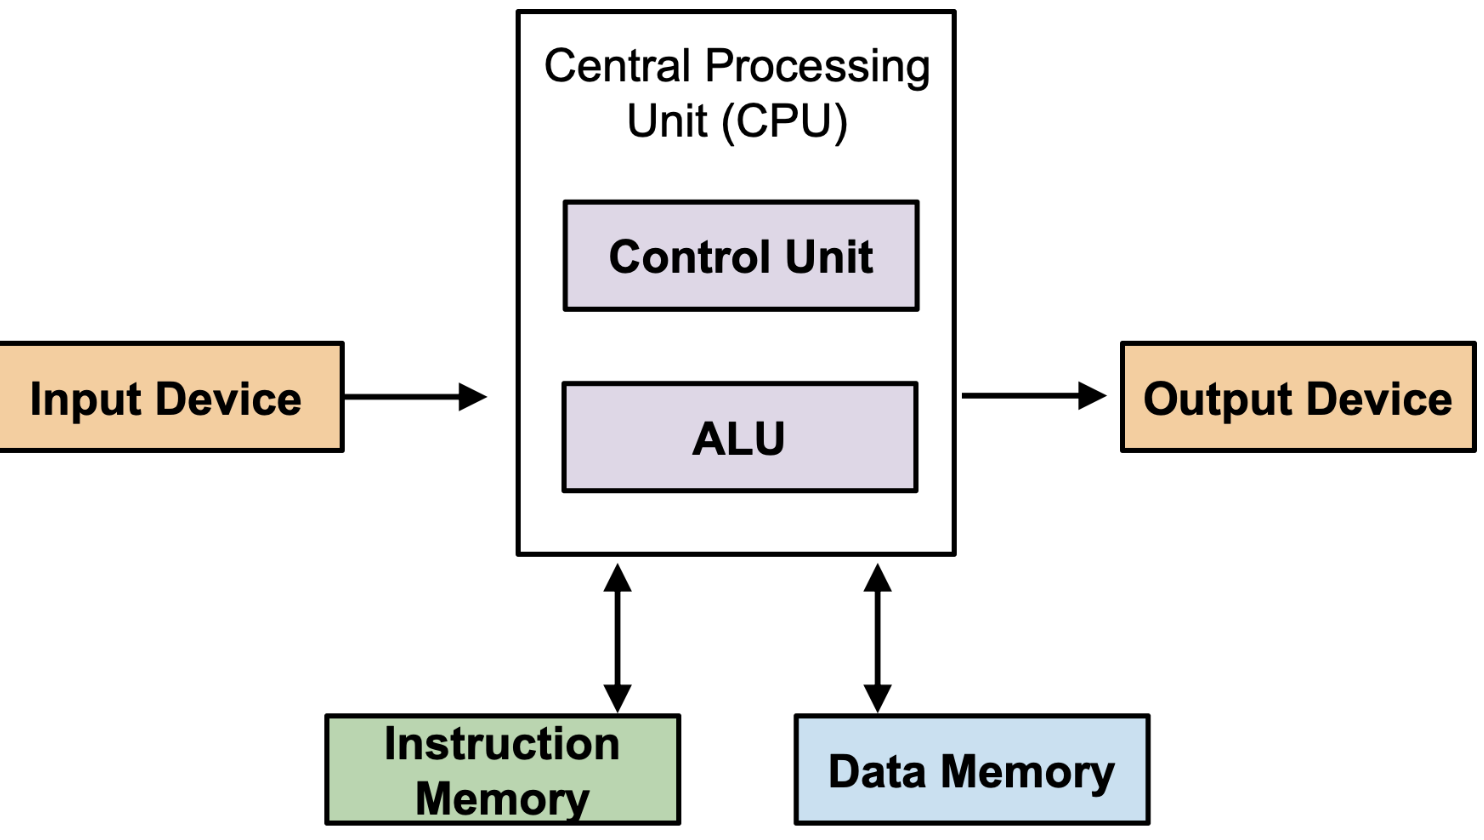
\includegraphics[scale=0.2]{harvard-architecture}
\subsubsection{Von Neumann architecture}
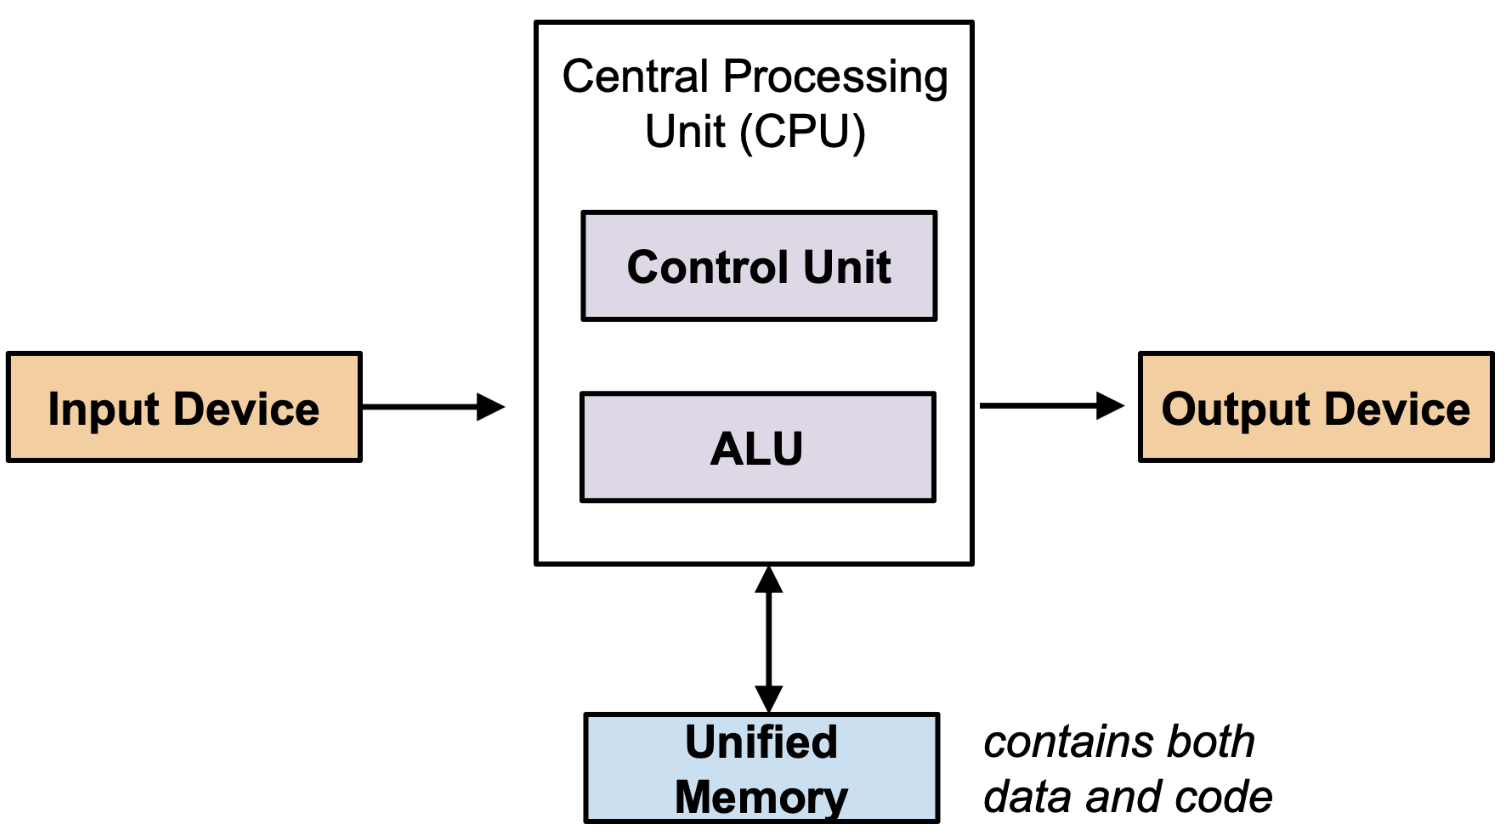
\includegraphics[scale=0.2]{von-neumann}

\begin{description}
	\item[Difference]{Separate vs common storage pathway for code and data}
\end{description}
Why do we need OS?

\subsection{Mainframe}
Old analog "computers" using physical cards for programming
\subsubsection{Improvements}
\begin{itemize}
	\item Problem: Batch processing inefficient
	\item Solution: Multiprogramming
	\begin{itemize}
		\item Loading multiple jobs that runs while other jobs using I/O
		\item Overlapping computation with I/O
	\end{itemize}
	\item Problem: Only one user 
	\item Solution: Time sharing OS
	\begin{itemize}
		\item Multiple concurrent users using terminals
		\item User job scheduling 
		\item Memory management
		\item \keyword{Hardware virtualization}{Each program executes as if it had all resources}
	\end{itemize}
\end{itemize}


\subsection{Motivation}
\begin{enumerate}
	\item Abstraction
	\begin{itemize}
		\item Hide low level details and present common, high-level functionality to users
	\end{itemize}
	\item Resource allocation
	\begin{itemize}
		\item Allow concurrent usage of resource and execute programs simultaneously
		\item Arbitrate conflicting request fairly and efficiently
	\end{itemize}
	\item Control programs
	\begin{itemize}
		\item Restrict resource allocation
		\item Security, protection and error prevention
		\item Ensure proper use of device
	\end{itemize}
\end{enumerate}
\subsubsection{Advantage}
\begin{itemize}
	\item Portable and flexible
	\item Use computer resources efficiently
\end{itemize}
\subsubsection{Disadvantage}
\begin{itemize}
	\item Significant overhead
\end{itemize}

\subsubsection{OS vs User Program}
Similarities
\begin{itemize}
	\item Both softwares
\end{itemize}
Difference
\begin{itemize}
	\item OS runs in \keyword{kernel mode}{Access to all hardware resources}
	\item User programs run in \keyword{User mode}{Limited access}
	\item User programs use syscalls to communicate with OS for hardware processes
\end{itemize}
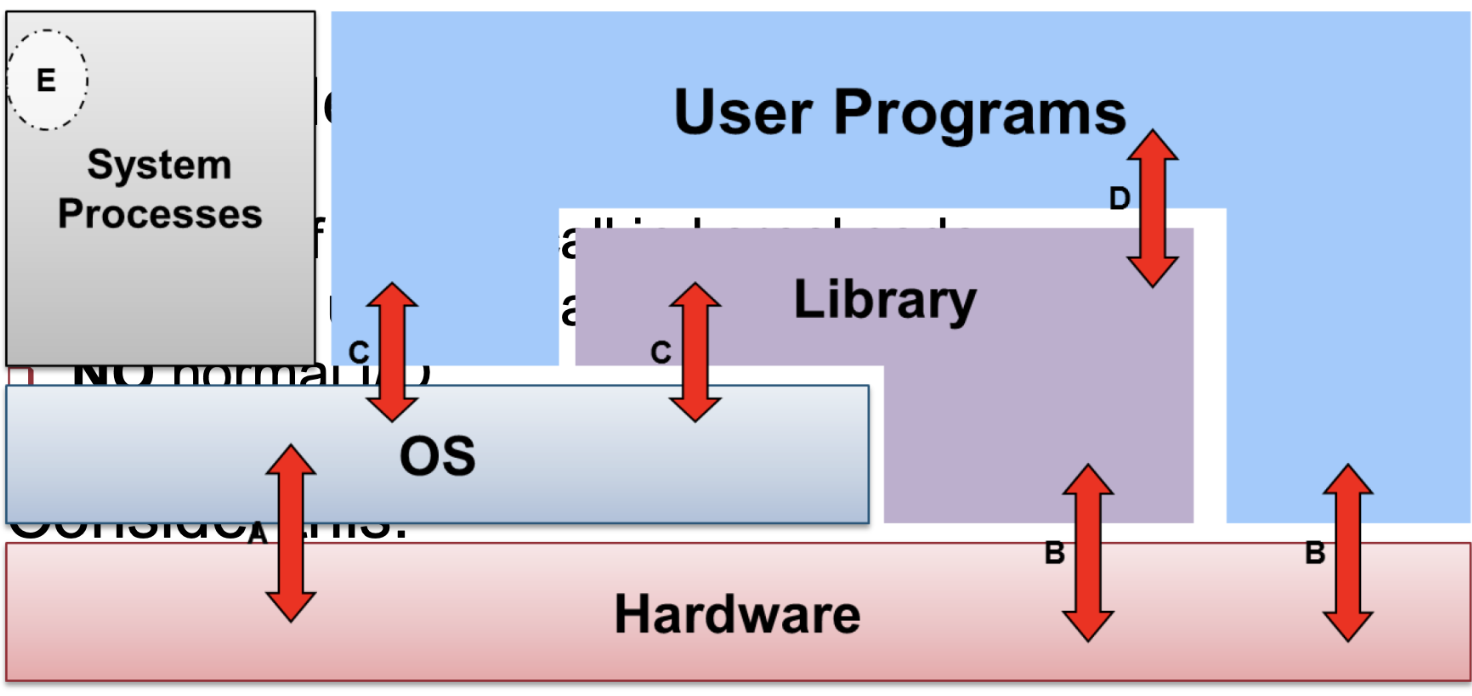
\includegraphics[scale=0.2]{os-interaction}
\\Why OS dont occupy entire hardware layer
\begin{itemize}
	\item Slow to have all operations pass through intermediary
	\item User programs can have direct interaction with hardware (eg. Arithmetic) during low risk operations
\end{itemize}

\subsection{OS structure}
\subsubsection{Monolithic OS}
\begin{itemize}
	\item One big kernel program
	\item Well understood and has good performance
	\item Highly \keyword{coupled}{internal structure interconnected that unintentionally affect each other}
\end{itemize}
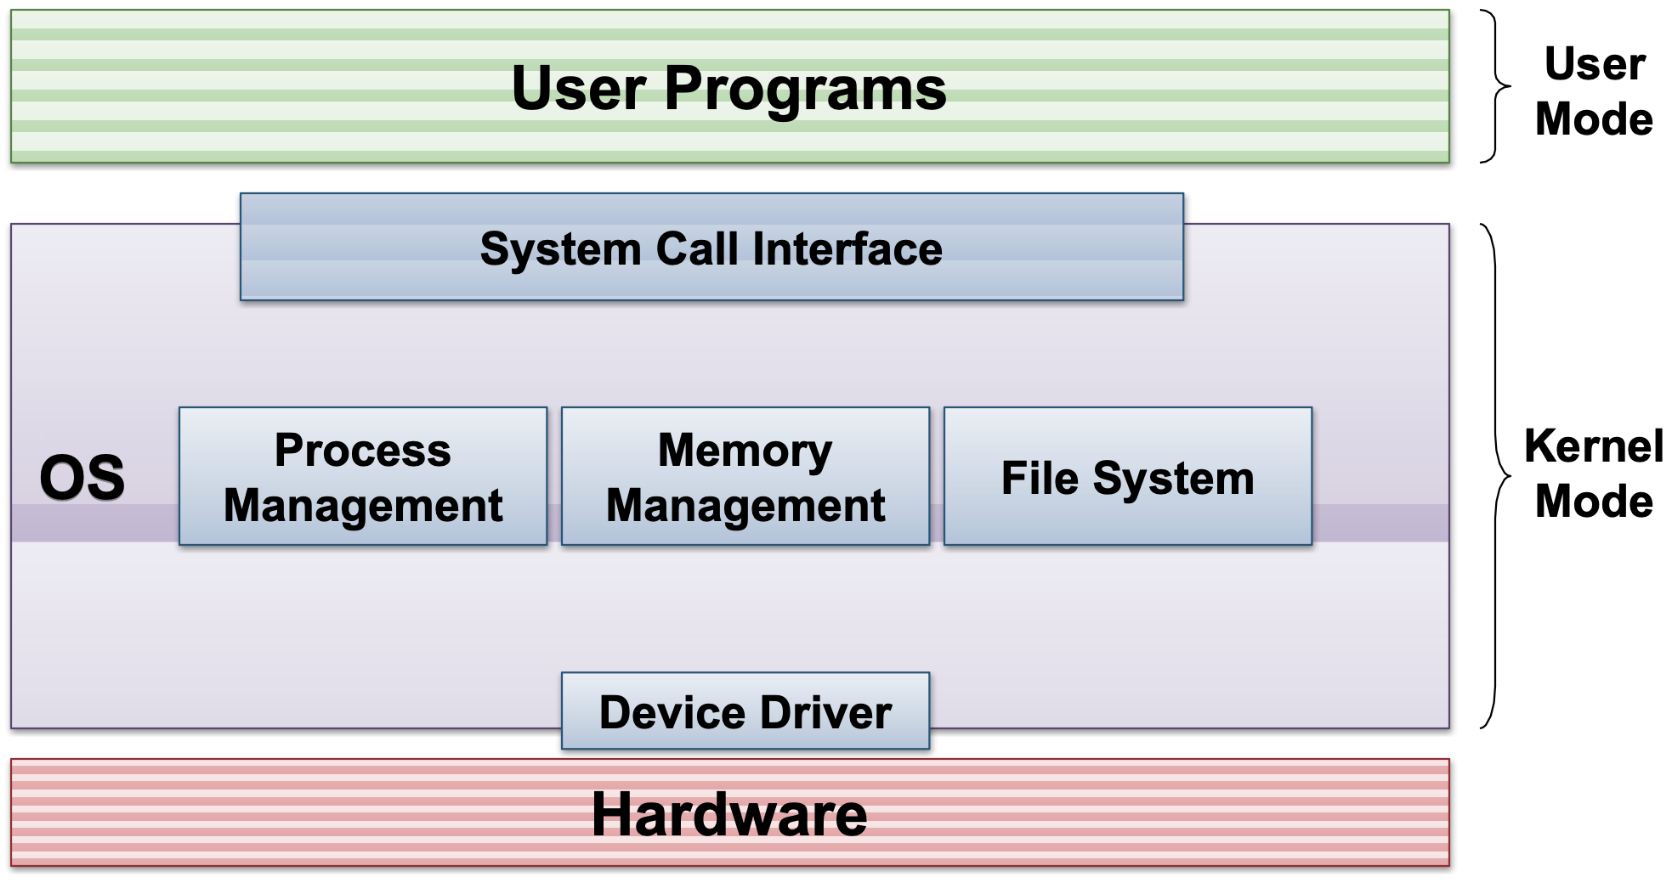
\includegraphics[scale=0.2]{monolithic-os}

\subsubsection{Microkernel}
\begin{itemize}
	\item Small clean
	\item Basic and essential facilities
	\item IPC communication OR run external programs outside OS
	\item Robust and more \keyword{modular}{Extendible and maintainable}
	\item Better isolation btw kernel and services
	\item Lower performance
\end{itemize}
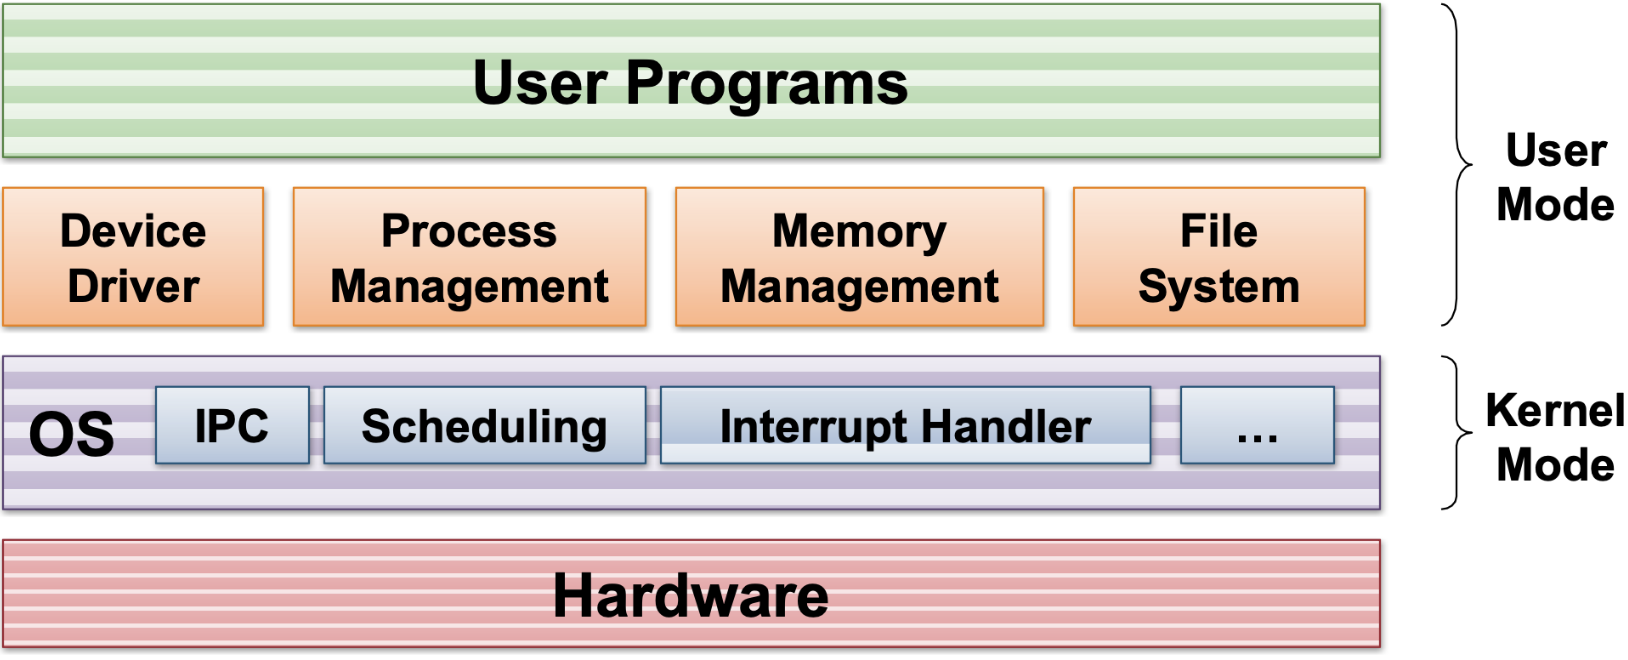
\includegraphics[scale=0.32]{microkernel-os}
%--------------------------------------------------------------------------------------------------------------------

\section{02. Process abstraction}
\subsection{Motivation}
\begin{itemize}
	\item Allow concurrent usage of hardware
	\item Multiple programs sharing the same processors/IO
\end{itemize}

\subsection{Computer organisation}
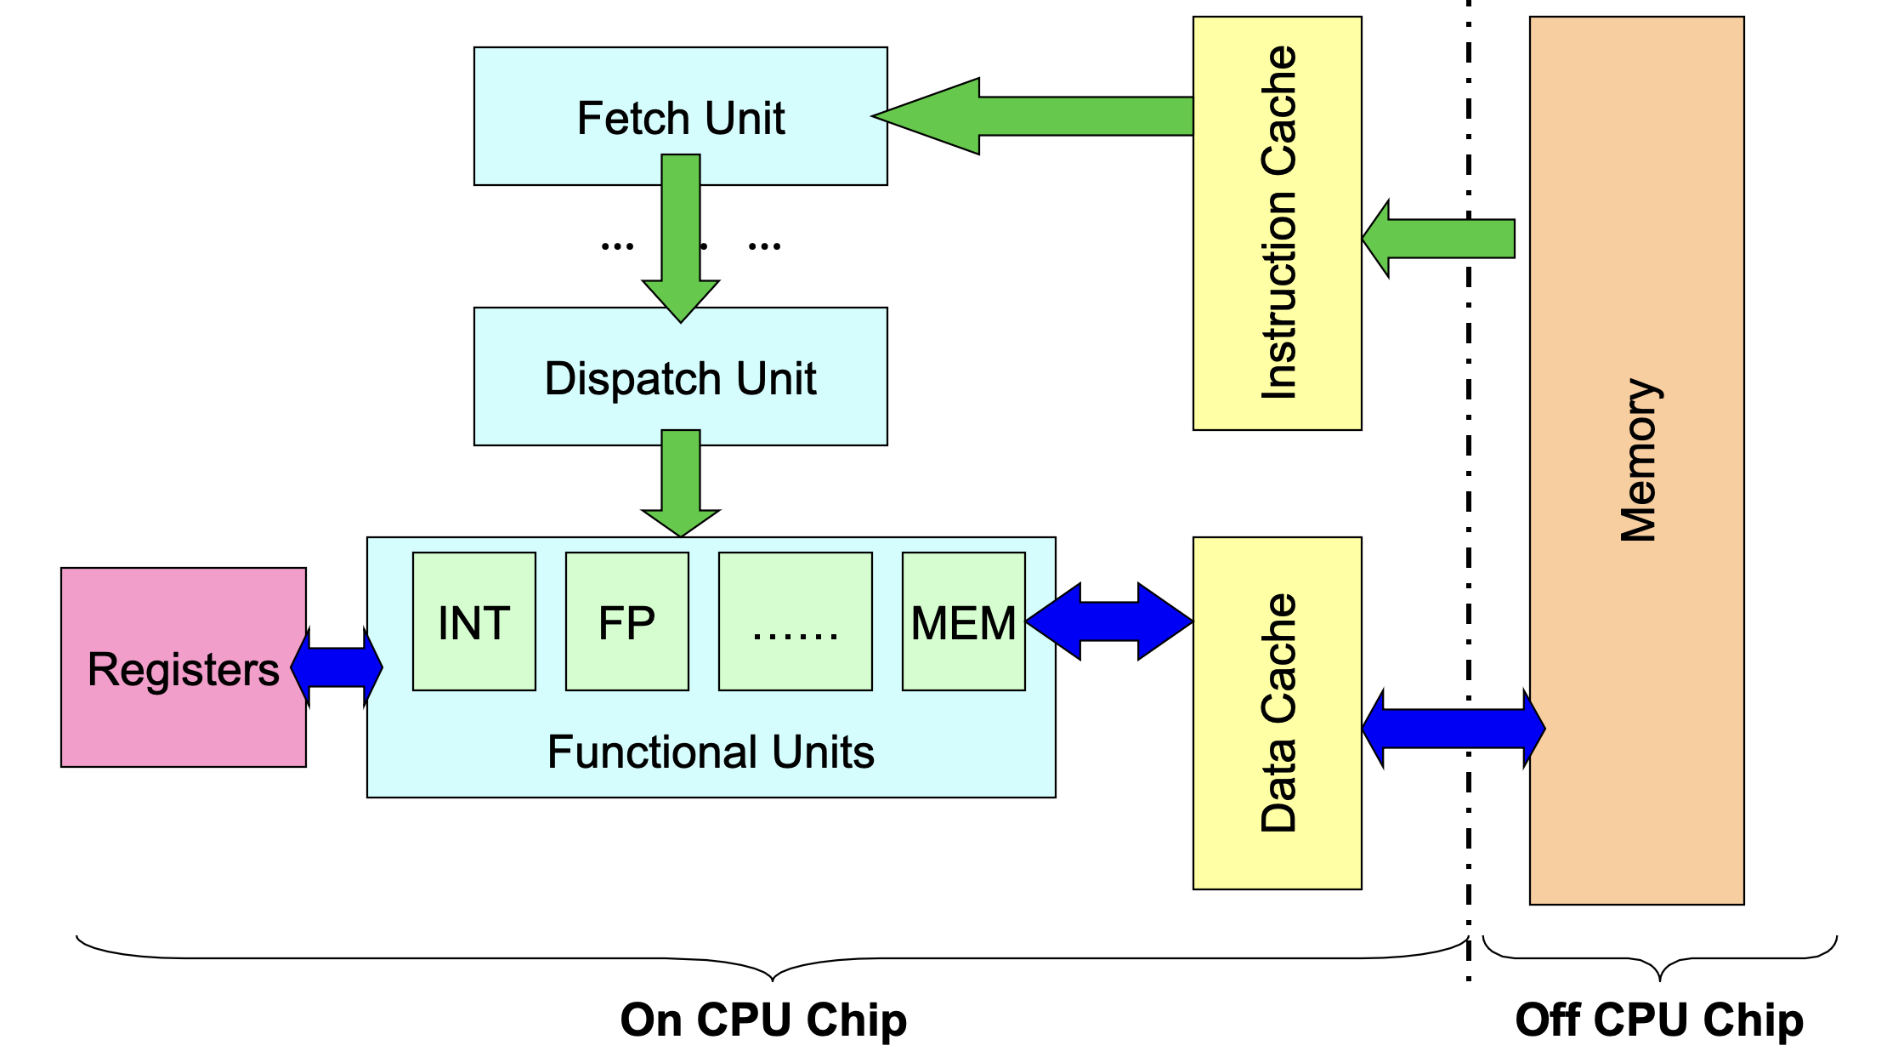
\includegraphics[scale=0.27]{computer-organisation}
\subsubsection{Memory}
\begin{itemize}
	\item Storage for instruction and data
	\item Managed by the OS
	\item Normally accessed via load/store instructions
\end{itemize}
\subsubsection{Cache}
\begin{itemize}
	\item Fast and invisible to software
	\item Duplicate part of the memory for faster access
	\item Usually split into instruction and data cache
\end{itemize}
\subsubsection{Fetch}
\begin{itemize}
	\item Load instructions from memory
	\item Location indicated by \textbf{Program Counter}
\end{itemize}
\subsubsection{Functional units}
\begin{itemize}
	\item Carry out instruction execution
	\item Dedicated to specific instruction type
\end{itemize}
\subsubsection{Registers}
\begin{itemize}
	\item Internal storage for fastest access speed
\end{itemize}

\subsection{Information needed}
\begin{itemize}
	\item Memory context
	\begin{itemize}
		\item Code
		\item Data
	\end{itemize}
	\item Hardware context
	\begin{itemize}
		\item Register
		\item PC value
		\item Frame Pointer
	\end{itemize}
	\item OS context
	\begin{itemize}
		\item Process properties
		\item Resources used
		\item Files
	\end{itemize}
\end{itemize}

\subsection{Function calls}
\subsubsection{Separation of text and data}
Suppose a function f() calls g()
\begin{itemize}
	\item f is caller and g is callee
\end{itemize}
Steps of control flow
\begin{enumerate}
	\item Setup parameters
	\item Trf ctrl to callee
	\item Setup local var
	\item Store any results
	\item Return ctrl to caller
\end{enumerate}
\subsubsection{Issues}
Control Flow
\begin{itemize}
	\item Need to jump to functional body when callee called
	\item Need to resume to next instruction in caller after done
\end{itemize}
Data storage
\begin{itemize}
	\item Need to pass parameters to function
	\item Need to capture return result
	\item May have local variables
\end{itemize}
Additional
\begin{itemize}
	\item May lead to overriding of data in caller by callee (interference)
	\item Calling g() multiple times may lead to insufficient space and overriding
\end{itemize}


\subsection{Stack memory}
Memory to store function invocation
\keyword{Stack Pointer}{Indicates the first free location in the stack region}\\
\keyword{Frame Pointer}{Points to the frame and is used for traversing around the stack easily}\\
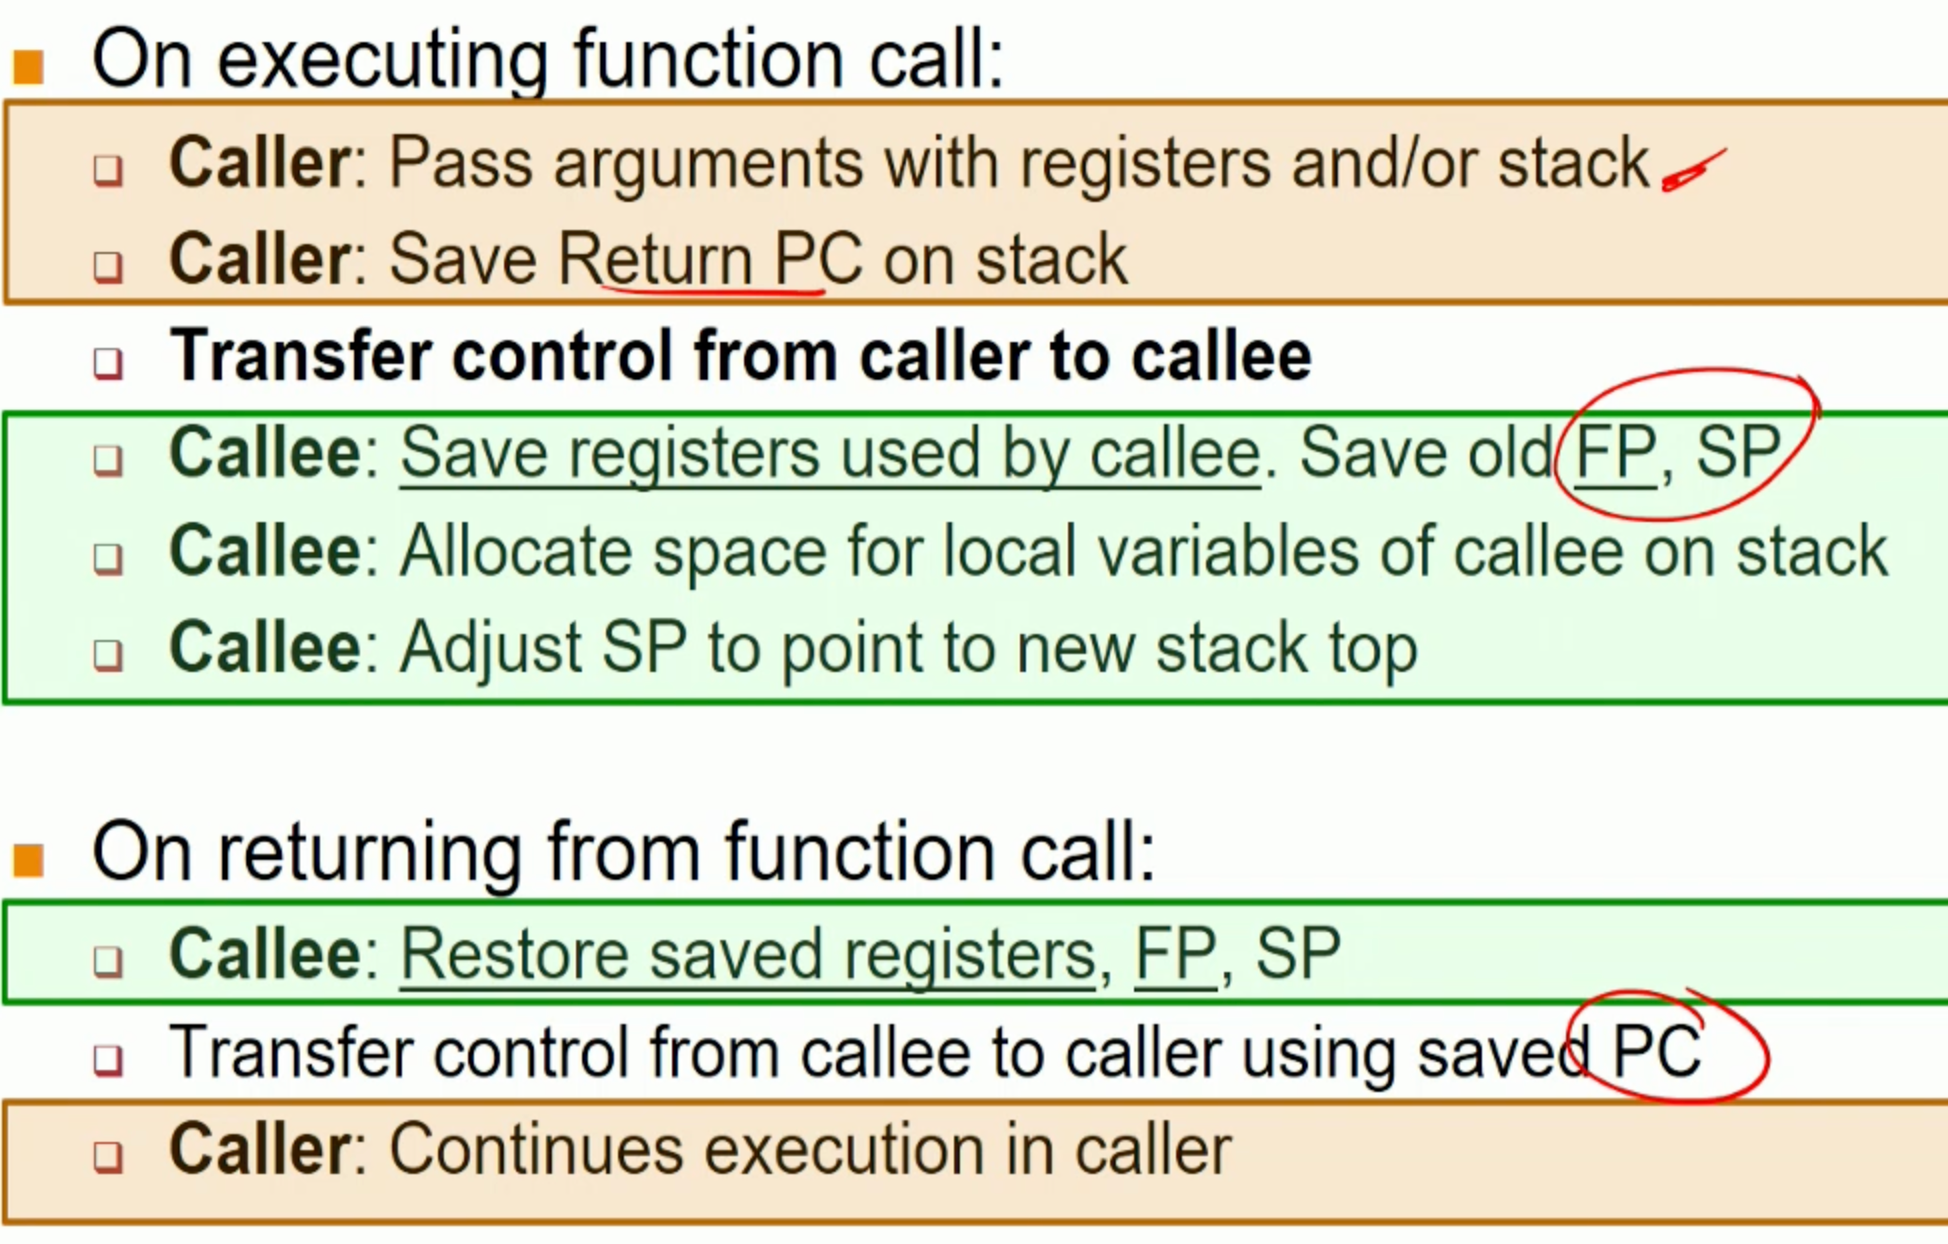
\includegraphics[scale=0.13]{stack-frame}\\
Information needed for function invocation - Stack frame
\begin{itemize}
	\item Return address of caller
	\item Arguments for the function
	\item Local variables
	\item Stack and frame pointer of caller
	\item GPR values (register spilling)
\end{itemize}
Callee stack frame will be on top of the caller


\subsection{Dynamic memory (Heap)}
Memory that the program/user specifies manually (eg. malloc, new)\\
Problems:
\begin{itemize}
	\item Allocated only at runtime
	\begin{itemize}
		\item Size not known at program compilation time
		\item Cannot specify a region in data 
	\end{itemize}
	\item No definite dellocation timing
	\begin{itemize}
		\item Must be freed explicitly by the program
		\item Cannot place in stack region
	\end{itemize}
\end{itemize}
Solution:\\
Add a region "Heap for dynamic allocation\\
Problems with heap memory:
\begin{itemize}
	\item Generation of holes in between data due to variable deallocation timing
\end{itemize}

%-----------------------------------------------------------------------------------------------------------------------
\subsection{OS context}
\subsubsection{Process identification}
Features:
\begin{itemize}
	\item Distinguish processes from each other (Unique)
	\item Communicated to the hardware
\end{itemize}
\subsubsection{Process state}
\begin{itemize}
	\item Denotes whether a process is running or not (Running vs waiting vs not running)
\end{itemize}
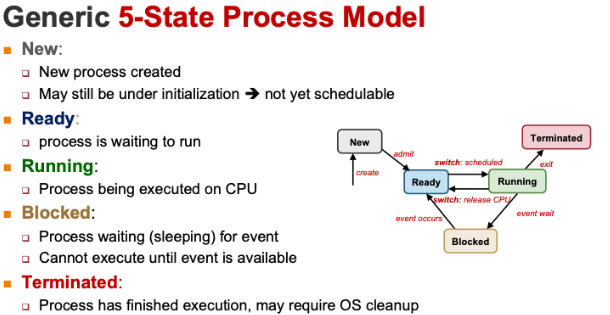
\includegraphics[scale=0.48]{process-model}

\keyword{Process control block}{Table representing all processes}

\subsection{Exceptions and interrupts}
Exceptions
\begin{itemize}
	\item Synchronous (due to program execution)
	\item Machine level instructions arise errors
	\item Exception handler executed automatically in software
\end{itemize}
Interrupts
\begin{itemize}
	\item Asynchronous (Can happen anytime)
	\item External events that cause execution to fail (hardware related errors)
	\item Program execution suspended and \textbf{interrupt handler} executed automatically
\end{itemize}

\subsubsection{Instruction execution}
\begin{enumerate}
	\item Read byte from PC and decode instruction
	\item Read 2 bytes to get the address/operands
	\item Perform ALU operations
	\item Store result into destination
	\item Check if any interruptions
\end{enumerate}
Interrupts can happen at anytime, and will remain pending until step 5 where it is handled

\subsubsection{Interruption handling}
\begin{enumerate}
	\item Push PC and status register into hardware
	\item Disable interrupts
	\item Read \keyword{Interrupt Vector Table}{Table where the OS stores address of all interrupt handlers}
	\item Switch to kernel mode
	\item Set PC to handler address and execute the instructions
\end{enumerate}
\begin{itemize}
	\item OS populates the IVT table with address of interrupt routines
	\item Hardware reads IVT to locate the handler
\end{itemize}

\subsection{System calls}
\keyword{Application Program Interface}{Provides way of calling facilities/services in kernel}\\
Instructions can only be done in kernel mode

\subsubsection{Method}
\begin{itemize}
	\item Library version with the same name and same arguments
	\item User friendly library version
	\item using the function $long~syscall(long~number);$
\end{itemize}
\subsubsection{Mechanism}
\begin{enumerate}
	\item User invoke library call
	\item Place call number in the designated location
	\item Library call executes a special instruction (\textbf{TRAP/syscall}) to change user to kernel mode
	\item (in kernel) syscall handler is determined (by a \textbf{dispatcher})
	\item syscall handler is executed
	\item Syscall handler ends and control returned to the library call
	\item Return to user mode and continue normal function mechanism
\end{enumerate}



%--------------------------------------------------------------------------------------------------------------------
%--------------------------------------------------------------------------------------------------------------------
%--------------------------------------------------------------------------------------------------------------------
%--------------------------------------------------------------------------------------------------------------------
\end{multicols*}
\end{document}
